% bare_jrnl.tex
%% V1.3
%% 2007/01/11
%% by Michael Shell
%% see http://www.michaelshell.org/
%% for current contact information.
%%
%% This is a skeleton file demonstrating the use of IEEEtran.cls
%% (requires IEEEtran.cls version 1.7 or later) with an IEEE journal paper.
%%
%% Support sites:
%% http://www.michaelshell.org/tex/ieeetran/
%% http://www.ctan.org/tex-archive/macros/latex/contrib/IEEEtran/
%% and
%% http://www.ieee.org/



% *** Authors should verify (and, if needed, correct) their LaTeX system  ***
% *** with the testflow diagnostic prior to trusting their LaTeX platform ***
% *** with production work. IEEE's font choices can trigger bugs that do  ***
% *** not appear when using other class files.                            ***
% The testflow support page is at:
% http://www.michaelshell.org/tex/testflow/


%%*************************************************************************
%% Legal Notice:
%% This code is offered as-is without any warranty either expressed or
%% implied; without even the implied warranty of MERCHANTABILITY or
%% FITNESS FOR A PARTICULAR PURPOSE! 
%% User assumes all risk.
%% In no event shall IEEE or any contributor to this code be liable for
%% any damages or losses, including, but not limited to, incidental,
%% consequential, or any other damages, resulting from the use or misuse
%% of any information contained here.
%%
%% All comments are the opinions of their respective authors and are not
%% necessarily endorsed by the IEEE.
%%
%% This work is distributed under the LaTeX Project Public License (LPPL)
%% ( http://www.latex-project.org/ ) version 1.3, and may be freely used,
%% distributed and modified. A copy of the LPPL, version 1.3, is included
%% in the base LaTeX documentation of all distributions of LaTeX released
%% 2003/12/01 or later.
%% Retain all contribution notices and credits.
%% ** Modified files should be clearly indicated as such, including  **
%% ** renaming them and changing author support contact information. **
%%
%% File list of work: IEEEtran.cls, IEEEtran_HOWTO.pdf, bare_adv.tex,
%%                    bare_conf.tex, bare_jrnl.tex, bare_jrnl_compsoc.tex
%%*************************************************************************

% Note that the a4paper option is mainly intended so that authors in
% countries using A4 can easily print to A4 and see how their papers will
% look in print - the typesetting of the document will not typically be
% affected with changes in paper size (but the bottom and side margins will).
% Use the testflow package mentioned above to verify correct handling of
% both paper sizes by the user's LaTeX system.
%
% Also note that the "draftcls" or "draftclsnofoot", not "draft", option
% should be used if it is desired that the figures are to be displayed in
% draft mode.
%
\documentclass[journal]{IEEEtran}
%
% If IEEEtran.cls has not been installed into the LaTeX system files,
% manually specify the path to it like:
% \documentclass[journal]{../sty/IEEEtran}





% Some very useful LaTeX packages include:
% (uncomment the ones you want to load)


% *** MISC UTILITY PACKAGES ***
%
%\usepackage{ifpdf}
% Heiko Oberdiek's ifpdf.sty is very useful if you need conditional
% compilation based on whether the output is pdf or dvi.
% usage:
% \ifpdf
%   % pdf code
% \else
%   % dvi code
% \fi
% The latest version of ifpdf.sty can be obtained from:
% http://www.ctan.org/tex-archive/macros/latex/contrib/oberdiek/
% Also, note that IEEEtran.cls V1.7 and later provides a builtin
% \ifCLASSINFOpdf conditional that works the same way.
% When switching from latex to pdflatex and vice-versa, the compiler may
% have to be run twice to clear warning/error messages.






% *** CITATION PACKAGES ***
%
%\usepackage{cite}
% cite.sty was written by Donald Arseneau
% V1.6 and later of IEEEtran pre-defines the format of the cite.sty package
% \cite{} output to follow that of IEEE. Loading the cite package will
% result in citation numbers being automatically sorted and properly
% "compressed/ranged". e.g., [1], [9], [2], [7], [5], [6] without using
% cite.sty will become [1], [2], [5]--[7], [9] using cite.sty. cite.sty's
% \cite will automatically add leading space, if needed. Use cite.sty's
% noadjust option (cite.sty V3.8 and later) if you want to turn this off.
% cite.sty is already installed on most LaTeX systems. Be sure and use
% version 4.0 (2003-05-27) and later if using hyperref.sty. cite.sty does
% not currently provide for hyperlinked citations.
% The latest version can be obtained at:
% http://www.ctan.org/tex-archive/macros/latex/contrib/cite/
% The documentation is contained in the cite.sty file itself.






% *** GRAPHICS RELATED PACKAGES ***
%
\ifCLASSINFOpdf
\usepackage[pdftex]{graphicx}
  % declare the path(s) where your graphic files are
  % \graphicspath{{../pdf/}{../jpeg/}}
  % and their extensions so you won't have to specify these with
  % every instance of \includegraphics
  % \DeclareGraphicsExtensions{.pdf,.jpeg,.png}
\else
  % or other class option (dvipsone, dvipdf, if not using dvips). graphicx
  % will default to the driver specified in the system graphics.cfg if no
  % driver is specified.
  % \usepackage[dvips]{graphicx}
  % declare the path(s) where your graphic files are
  % \graphicspath{{../eps/}}
  % and their extensions so you won't have to specify these with
  % every instance of \includegraphics
  % \DeclareGraphicsExtensions{.eps}
\fi
% graphicx was written by David Carlisle and Sebastian Rahtz. It is
% required if you want graphics, photos, etc. graphicx.sty is already
% installed on most LaTeX systems. The latest version and documentation can
% be obtained at: 
% http://www.ctan.org/tex-archive/macros/latex/required/graphics/
% Another good source of documentation is "Using Imported Graphics in
% LaTeX2e" by Keith Reckdahl which can be found as epslatex.ps or
% epslatex.pdf at: http://www.ctan.org/tex-archive/info/
%
% latex, and pdflatex in dvi mode, support graphics in encapsulated
% postscript (.eps) format. pdflatex in pdf mode supports graphics
% in .pdf, .jpeg, .png and .mps (metapost) formats. Users should ensure
% that all non-photo figures use a vector format (.eps, .pdf, .mps) and
% not a bitmapped formats (.jpeg, .png). IEEE frowns on bitmapped formats
% which can result in "jaggedy"/blurry rendering of lines and letters as
% well as large increases in file sizes.
%
% You can find documentation about the pdfTeX application at:
% http://www.tug.org/applications/pdftex





% *** MATH PACKAGES ***
%
%\usepackage[cmex10]{amsmath}
% A popular package from the American Mathematical Society that provides
% many useful and powerful commands for dealing with mathematics. If using
% it, be sure to load this package with the cmex10 option to ensure that
% only type 1 fonts will utilized at all point sizes. Without this option,
% it is possible that some math symbols, particularly those within
% footnotes, will be rendered in bitmap form which will result in a
% document that can not be IEEE Xplore compliant!
%
% Also, note that the amsmath package sets \interdisplaylinepenalty to 10000
% thus preventing page breaks from occurring within multiline equations. Use:
%\interdisplaylinepenalty=2500
% after loading amsmath to restore such page breaks as IEEEtran.cls normally
% does. amsmath.sty is already installed on most LaTeX systems. The latest
% version and documentation can be obtained at:
% http://www.ctan.org/tex-archive/macros/latex/required/amslatex/math/





% *** SPECIALIZED LIST PACKAGES ***
%
%\usepackage{algorithmic}
% algorithmic.sty was written by Peter Williams and Rogerio Brito.
% This package provides an algorithmic environment fo describing algorithms.
% You can use the algorithmic environment in-text or within a figure
% environment to provide for a floating algorithm. Do NOT use the algorithm
% floating environment provided by algorithm.sty (by the same authors) or
% algorithm2e.sty (by Christophe Fiorio) as IEEE does not use dedicated
% algorithm float types and packages that provide these will not provide
% correct IEEE style captions. The latest version and documentation of
% algorithmic.sty can be obtained at:
% http://www.ctan.org/tex-archive/macros/latex/contrib/algorithms/
% There is also a support site at:
% http://algorithms.berlios.de/index.html
% Also of interest may be the (relatively newer and more customizable)
% algorithmicx.sty package by Szasz Janos:
% http://www.ctan.org/tex-archive/macros/latex/contrib/algorithmicx/




% *** ALIGNMENT PACKAGES ***
%
%\usepackage{array}
% Frank Mittelbach's and David Carlisle's array.sty patches and improves
% the standard LaTeX2e array and tabular environments to provide better
% appearance and additional user controls. As the default LaTeX2e table
% generation code is lacking to the point of almost being broken with
% respect to the quality of the end results, all users are strongly
% advised to use an enhanced (at the very least that provided by array.sty)
% set of table tools. array.sty is already installed on most systems. The
% latest version and documentation can be obtained at:
% http://www.ctan.org/tex-archive/macros/latex/required/tools/


%\usepackage{mdwmath}
%\usepackage{mdwtab}
% Also highly recommended is Mark Wooding's extremely powerful MDW tools,
% especially mdwmath.sty and mdwtab.sty which are used to format equations
% and tables, respectively. The MDWtools set is already installed on most
% LaTeX systems. The lastest version and documentation is available at:
% http://www.ctan.org/tex-archive/macros/latex/contrib/mdwtools/


% IEEEtran contains the IEEEeqnarray family of commands that can be used to
% generate multiline equations as well as matrices, tables, etc., of high
% quality.


%\usepackage{eqparbox}
% Also of notable interest is Scott Pakin's eqparbox package for creating
% (automatically sized) equal width boxes - aka "natural width parboxes".
% Available at:
% http://www.ctan.org/tex-archive/macros/latex/contrib/eqparbox/





% *** SUBFIGURE PACKAGES ***
%\usepackage[tight,footnotesize]{subfigure}
% subfigure.sty was written by Steven Douglas Cochran. This package makes it
% easy to put subfigures in your figures. e.g., "Figure 1a and 1b". For IEEE
% work, it is a good idea to load it with the tight package option to reduce
% the amount of white space around the subfigures. subfigure.sty is already
% installed on most LaTeX systems. The latest version and documentation can
% be obtained at:
% http://www.ctan.org/tex-archive/obsolete/macros/latex/contrib/subfigure/
% subfigure.sty has been superceeded by subfig.sty.



%\usepackage[caption=false]{caption}
%\usepackage[font=footnotesize]{subfig}
% subfig.sty, also written by Steven Douglas Cochran, is the modern
% replacement for subfigure.sty. However, subfig.sty requires and
% automatically loads Axel Sommerfeldt's caption.sty which will override
% IEEEtran.cls handling of captions and this will result in nonIEEE style
% figure/table captions. To prevent this problem, be sure and preload
% caption.sty with its "caption=false" package option. This is will preserve
% IEEEtran.cls handing of captions. Version 1.3 (2005/06/28) and later 
% (recommended due to many improvements over 1.2) of subfig.sty supports
% the caption=false option directly:
%\usepackage[caption=false,font=footnotesize]{subfig}
%
% The latest version and documentation can be obtained at:
% http://www.ctan.org/tex-archive/macros/latex/contrib/subfig/
% The latest version and documentation of caption.sty can be obtained at:
% http://www.ctan.org/tex-archive/macros/latex/contrib/caption/




% *** FLOAT PACKAGES ***
%
%\usepackage{fixltx2e}
% fixltx2e, the successor to the earlier fix2col.sty, was written by
% Frank Mittelbach and David Carlisle. This package corrects a few problems
% in the LaTeX2e kernel, the most notable of which is that in current
% LaTeX2e releases, the ordering of single and double column floats is not
% guaranteed to be preserved. Thus, an unpatched LaTeX2e can allow a
% single column figure to be placed prior to an earlier double column
% figure. The latest version and documentation can be found at:
% http://www.ctan.org/tex-archive/macros/latex/base/



%\usepackage{stfloats}
% stfloats.sty was written by Sigitas Tolusis. This package gives LaTeX2e
% the ability to do double column floats at the bottom of the page as well
% as the top. (e.g., "\begin{figure*}[!b]" is not normally possible in
% LaTeX2e). It also provides a command:
%\fnbelowfloat
% to enable the placement of footnotes below bottom floats (the standard
% LaTeX2e kernel puts them above bottom floats). This is an invasive package
% which rewrites many portions of the LaTeX2e float routines. It may not work
% with other packages that modify the LaTeX2e float routines. The latest
% version and documentation can be obtained at:
% http://www.ctan.org/tex-archive/macros/latex/contrib/sttools/
% Documentation is contained in the stfloats.sty comments as well as in the
% presfull.pdf file. Do not use the stfloats baselinefloat ability as IEEE
% does not allow \baselineskip to stretch. Authors submitting work to the
% IEEE should note that IEEE rarely uses double column equations and
% that authors should try to avoid such use. Do not be tempted to use the
% cuted.sty or midfloat.sty packages (also by Sigitas Tolusis) as IEEE does
% not format its papers in such ways.


%\ifCLASSOPTIONcaptionsoff
%  \usepackage[nomarkers]{endfloat}
% \let\MYoriglatexcaption\caption
% \renewcommand{\caption}[2][\relax]{\MYoriglatexcaption[#2]{#2}}
%\fi
% endfloat.sty was written by James Darrell McCauley and Jeff Goldberg.
% This package may be useful when used in conjunction with IEEEtran.cls'
% captionsoff option. Some IEEE journals/societies require that submissions
% have lists of figures/tables at the end of the paper and that
% figures/tables without any captions are placed on a page by themselves at
% the end of the document. If needed, the draftcls IEEEtran class option or
% \CLASSINPUTbaselinestretch interface can be used to increase the line
% spacing as well. Be sure and use the nomarkers option of endfloat to
% prevent endfloat from "marking" where the figures would have been placed
% in the text. The two hack lines of code above are a slight modification of
% that suggested by in the endfloat docs (section 8.3.1) to ensure that
% the full captions always appear in the list of figures/tables - even if
% the user used the short optional argument of \caption[]{}.
% IEEE papers do not typically make use of \caption[]'s optional argument,
% so this should not be an issue. A similar trick can be used to disable
% captions of packages such as subfig.sty that lack options to turn off
% the subcaptions:
% For subfig.sty:
% \let\MYorigsubfloat\subfloat
% \renewcommand{\subfloat}[2][\relax]{\MYorigsubfloat[]{#2}}
% For subfigure.sty:
% \let\MYorigsubfigure\subfigure
% \renewcommand{\subfigure}[2][\relax]{\MYorigsubfigure[]{#2}}
% However, the above trick will not work if both optional arguments of
% the \subfloat/subfig command are used. Furthermore, there needs to be a
% description of each subfigure *somewhere* and endfloat does not add
% subfigure captions to its list of figures. Thus, the best approach is to
% avoid the use of subfigure captions (many IEEE journals avoid them anyway)
% and instead reference/explain all the subfigures within the main caption.
% The latest version of endfloat.sty and its documentation can obtained at:
% http://www.ctan.org/tex-archive/macros/latex/contrib/endfloat/
%
% The IEEEtran \ifCLASSOPTIONcaptionsoff conditional can also be used
% later in the document, say, to conditionally put the References on a 
% page by themselves.





% *** PDF, URL AND HYPERLINK PACKAGES ***
%
%\usepackage{url}
% url.sty was written by Donald Arseneau. It provides better support for
% handling and breaking URLs. url.sty is already installed on most LaTeX
% systems. The latest version can be obtained at:
% http://www.ctan.org/tex-archive/macros/latex/contrib/misc/
% Read the url.sty source comments for usage information. Basically,
% \url{my_url_here}.





% *** Do not adjust lengths that control margins, column widths, etc. ***
% *** Do not use packages that alter fonts (such as pslatex).         ***
% There should be no need to do such things with IEEEtran.cls V1.6 and later.
% (Unless specifically asked to do so by the journal or conference you plan
% to submit to, of course. )


% correct bad hyphenation here
\hyphenation{}


\begin{document}
\pagenumbering{gobble}
%
% paper title
% can use linebreaks \\ within to get better formatting as desired
\title{The CMS Data Quality Monitoring Software: Experience and Future Improvements}
%
%
% author names and IEEE memberships
% note positions of commas and nonbreaking spaces ( ~ ) LaTeX will not break
% a structure at a ~ so this keeps an author's name from being broken across
% two lines.
% use \thanks{} to gain access to the first footnote area
% a separate \thanks must be used for each paragraph as LaTeX2e's \thanks
% was not built to handle multiple paragraphs
%

\author{Atanas~Batinkov,
		Marco~Rovere,
		Laura~Borrello,
		Federico~De~Guio,
		Daniel~Duggan,
		and~Salvatore~Di~Guida on behalf of the CMS Collaboration% <-this % stops a space        
\thanks{A. Batinkov is with the University of Sofia (BG).}% <-this % stops a space
\thanks{M. Rovere is with CERN.}% <-this % stops a space
\thanks{L. Borrello is with the University of Wisconsin (US).}% <-this % stops a space
\thanks{F. De Guio is with CERN.}% <-this % stops a space
\thanks{D. Duggan is with the Rutgers, State Univ. of New Jersey (US).}% <-this % stops a space
\thanks{S. Di Guida is with the Universita degli Studi Guglielmo Marconi (IT).}}% <-this % stops a space

% note the % following the last \IEEEmembership and also \thanks - 
% these prevent an unwanted space from occurring between the last author name
% and the end of the author line. i.e., if you had this:
% 
% \author{....lastname \thanks{...} \thanks{...} }
%                     ^------------^------------^----Do not want these spaces!
%
% a space would be appended to the last name and could cause every name on that
% line to be shifted left slightly. This is one of those "LaTeX things". For
% instance, "\textbf{A} \textbf{B}" will typeset as "A B" not "AB". To get
% "AB" then you have to do: "\textbf{A}\textbf{B}"
% \thanks is no different in this regard, so shield the last } of each \thanks
% that ends a line with a % and do not let a space in before the next \thanks.
% Spaces after \IEEEmembership other than the last one are OK (and needed) as
% you are supposed to have spaces between the names. For what it is worth,
% this is a minor point as most people would not even notice if the said evil
% space somehow managed to creep in.



% The paper headers
%\markboth{Journal of \LaTeX\ Class Files,~Vol.~6, No.~1, January~2007}%
%{Shell \MakeLowercase{\textit{et al.}}: Bare Demo of IEEEtran.cls for Journals}
% The only time the second header will appear is for the odd numbered pages
% after the title page when using the twoside option.
% 
% *** Note that you probably will NOT want to include the author's ***
% *** name in the headers of peer review papers.                   ***
% You can use \ifCLASSOPTIONpeerreview for conditional compilation here if
% you desire.




% If you want to put a publisher's ID mark on the page you can do it like
% this:
%\IEEEpubid{0000--0000/00\$00.00~\copyright~2007 IEEE}
% Remember, if you use this you must call \IEEEpubidadjcol in the second
% column for its text to clear the IEEEpubid mark.



% use for special paper notices
%\IEEEspecialpapernotice{(Invited Paper)}




% make the title area
\maketitle


\begin{abstract}
%\boldmath
The Data Quality Monitoring Software proved to be a central tool in the Compact Muon Solenoid experiment. Its flexibility allowed its integration in several environments: online, for real-time detector monitoring; offline, for the final, fine-grained data certification. The usage of the Data Quality Monitoring software in the different environments and its integration in the Compact Muon Solenoid reconstruction software framework and in all production work-flows are presented. The main technical challenges and the adopted solutions to them will be also discussed with emphasis on functionality, longterm robustness and performance.
\end{abstract}
% IEEEtran.cls defaults to using nonbold math in the Abstract.
% This preserves the distinction between vectors and scalars. However,
% if the journal you are submitting to favors bold math in the abstract,
% then you can use LaTeX's standard command \boldmath at the very start
% of the abstract to achieve this. Many IEEE journals frown on math
% in the abstract anyway.

% Note that keywords are not normally used for peerreview papers.
% \begin{IEEEkeywords}
% IEEEtran, journal, \LaTeX, paper, template.
% \end{IEEEkeywords}






% For peer review papers, you can put extra information on the cover
% page as needed:
% \ifCLASSOPTIONpeerreview
% \begin{center} \bfseries EDICS Category: 3-BBND \end{center}
% \fi
%
% For peerreview papers, this IEEEtran command inserts a page break and
% creates the second title. It will be ignored for other modes.
\IEEEpeerreviewmaketitle



\section{Introduction}
% The very first letter is a 2 line initial drop letter followed
% by the rest of the first word in caps.
% 
% form to use if the first word consists of a single letter:
% \IEEEPARstart{A}{demo} file is ....
% 
% form to use if you need the single drop letter followed by
% normal text (unknown if ever used by IEEE):
% \IEEEPARstart{A}{}demo file is ....
% 
% Some journals put the first two words in caps:
% \IEEEPARstart{T}{his demo} file is ....
% 
% Here we have the typical use of a "T" for an initial drop letter
% and "HIS" in caps to complete the first word.
\IEEEPARstart{T}{he} Large Hadron Collider (LHC) \cite{LHC} at CERN \cite{CERN} collides protons together at close to the speed of light. Some of the collision energy is turned into mass, creating new particles which are observed in the Compact Muon Solenoid (CMS) \cite{CMS} particle detector. CMS data is analyzed by physicists around the world to reconstruct a picture of what happened at the heart of these collisions. Data quality monitoring (DQM) is a crucial part of the experiment. Its purpose is to identify errors and problems in the detector hardware or reconstruction software. The ultimate goal is a stable detector leading to high quality reconstructed collision events. There are two main branches of the monitoring framework, online and offline, and each is discussed in detail below.
% You must have at least 2 lines in the paragraph with the drop letter
% (should never be an issue)

\section{DQM online realm}
The online DQM is responsible for identifying problems with detector performance and data integrity during data-taking periods (runs). This is real-time data monitoring, fast response time periods to identify serious issues coming from detector problems or running conditions. The objective is to minimize the recording of bad data by giving instant feedback to experts (Fig. \ref{fig:OnlineChain}).

\begin{figure}
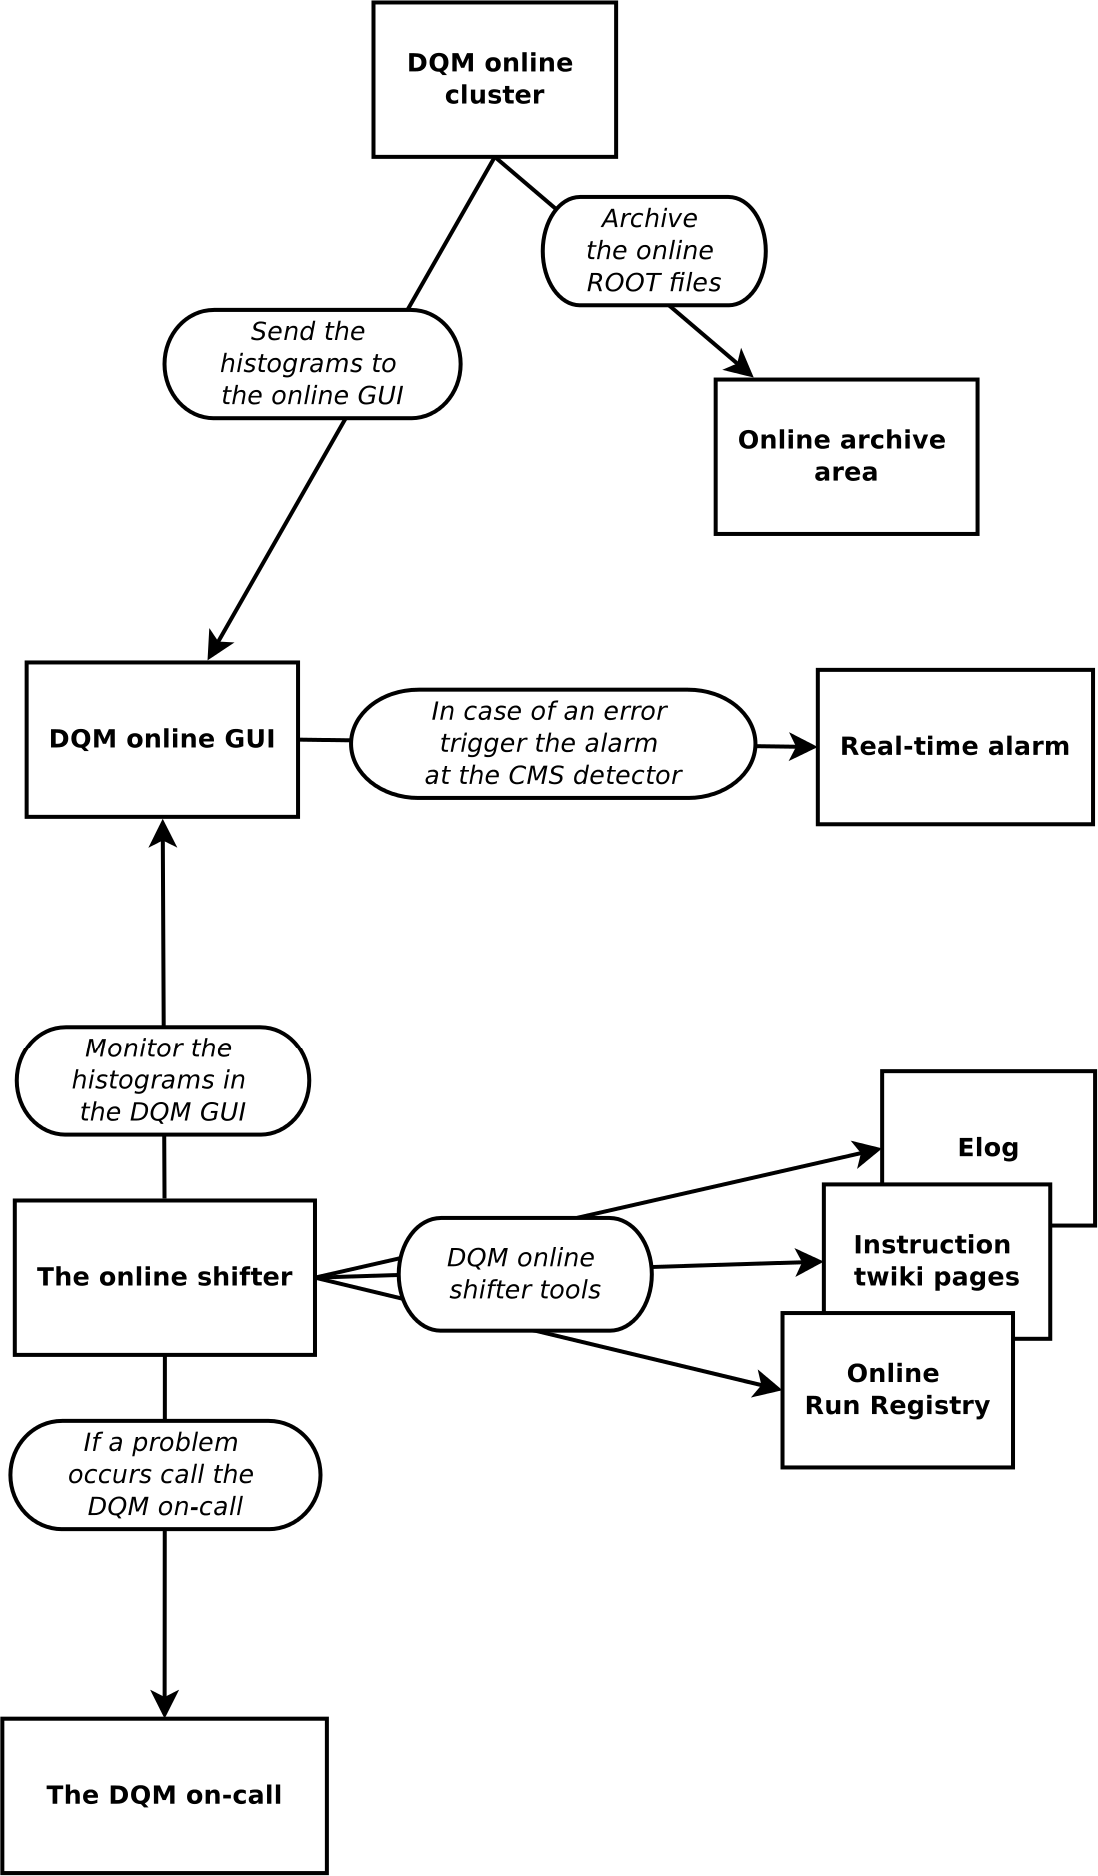
\includegraphics[width=0.5\textwidth, keepaspectratio=true]{OnlineChain.png}
\caption{The DQM online chain. This figure outlines the 3 main aspects of the online realm: the online cluster and the archive area, the online DQM GUI and the sound alarm, the online shifter}
\label{fig:OnlineChain}
\end{figure}

\subsection{DQM online cluster \& the archive area}
The DQM online cluster processes live data and produces histograms that are used to identify problems during the data-taking. It hosts the DQM framework, part of the CMS software framework (CMSSW). All detector subsystems have their own online monitoring applications run centrally through the DQM framework. They produce real-time histograms that are transferred to the DQM GUI over the local network. New software from the detector subsystems is deployed on demand twice a week so all the subsystems can keep their applications up to date under this flexible and responsive scheme. To ensure stability, all software changes are tested and verified in an online replica cluster for a 24hr period before they are deployed at the production machines.

All the produced histograms are periodically archived as ROOT \cite{ROOT} files for a continuous backup in the online archive area. This archive is used in the rare case of a DQM GUI database failure. If this happens, the online ROOT files from the archive area can be injected into the DQM GUI in order to restore the database.

\subsection{DQM online GUI \& the sound alarm}
\label{sec:OnlineGUI}
The online DQM GUI (Fig. \ref{fig:OnlineGUI}) collects, stores, and visualizes the results from the online applications. It is web based, which makes it OS independent and accessible from everywhere around the world. It is almost completely decoupled from the CMSSW, which makes it easy to install. The GUI has its own key-value database called ’index’ to store the serialized histogram data. The ROOT framework is used to render the data from the index to histograms. This process is detached from the server which also guarantees stability in case of a ROOT crash. The DQM GUI allows customizations. Users from the detector subsystems can define different workspaces, layouts and render plug-ins for their histogram sets. The GUI also has rich web API that supports JSON format. Everything that the user needs can be retrieved from the server in serialized JSON format. In order to benefit from the GUI customization abilities the DQM team provides flexible schema for new software deployment.

\begin{figure}
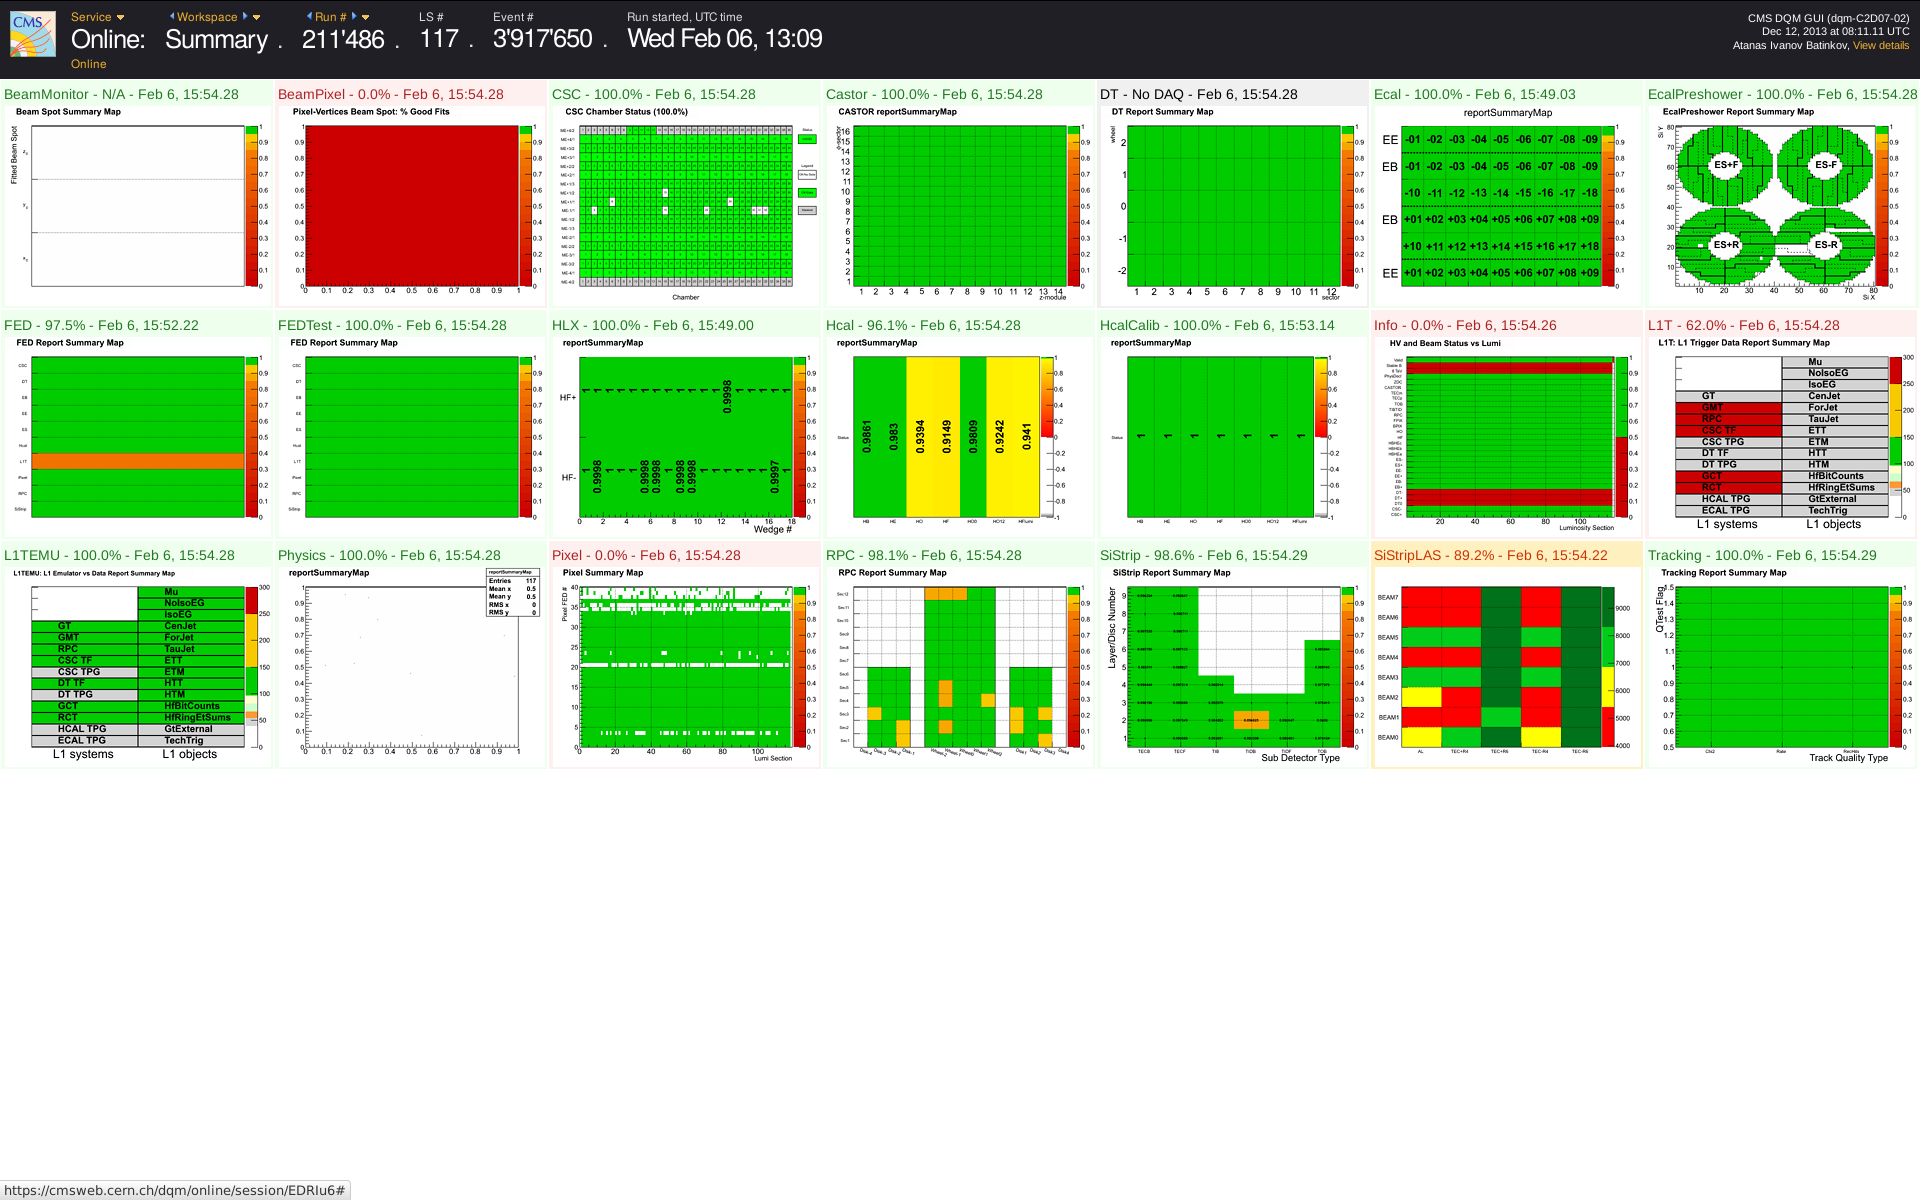
\includegraphics[width=0.5\textwidth, keepaspectratio=true]{OnlineGUI.png}
\caption{The DQM online GUI. This picture shows the summary workspace.}
\label{fig:OnlineGUI}
\end{figure}

A real-time alarm system to alert shifters and experts at the detector of potential issues and the quality of the recorded data is used. It indicates critical problems and maximizes good quality data during data taking. Customized histograms provided from subsystems act as triggers to identify critical problems. These histograms are hosted in a dedicated central location in the online GUI mapped to the audio alarm for the shift crew.

\subsection{Online shifter \& the DQM on-call}
\label{sec:OnlineShifter}
The scope of the DQM online shift is to identify problems with detector performance and data integrity during the run. Shifts take place at the CMS control room on the site of the detector. Dedicated DQM shifts are scheduled 24/7 in data taking periods. There are 3 shifts per day and each takes 8 hours. The online shifter monitors a subset of histograms for every detector and reconstruction objects in the DQM GUI. The tools of the online DQM shifter are: the DQM GUI, the twiki pages, online Run Registry (Fig. \ref{fig:OnlineRunRegistry}) and the Elog (Fig. \ref{fig:Elog}). The Twiki Pages provide a comprehensive set of instructions of how to evaluate individual histograms, and what steps to take in case of problems. The Run Registry is a web-based bookkeeping tool that collects information about all the significant runs and the data certification results from those runs. The Elog is a central logging system where all parties can leave comments and report issues, among many other use cases.

\begin{figure}
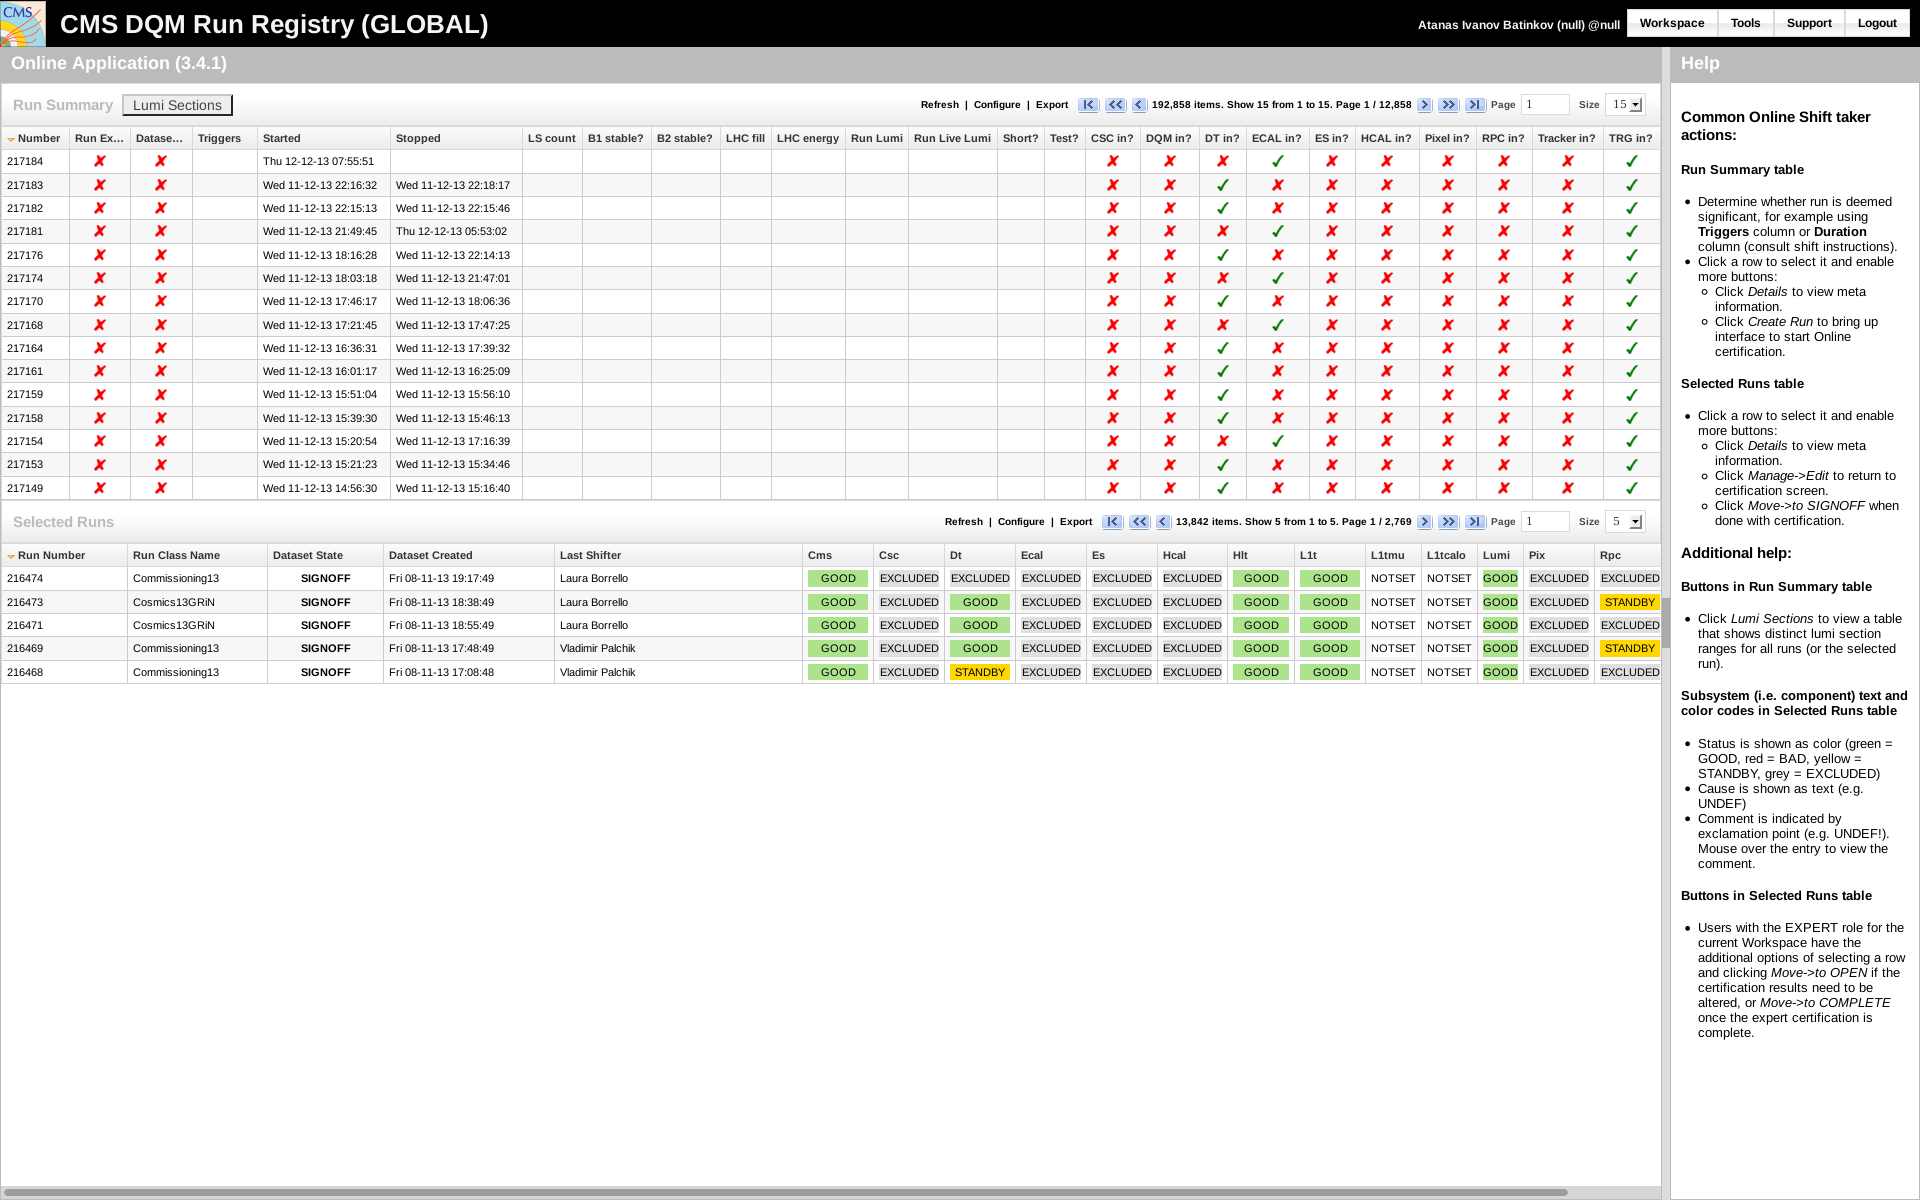
\includegraphics[width=0.5\textwidth, keepaspectratio=true]{OnlineRunRegistry.png}
\caption{Online Run Registry. On the top you can see the list of runs waiting to be certified. On the bottom is the list of certified runs.}
\label{fig:OnlineRunRegistry}
\end{figure}

\begin{figure}
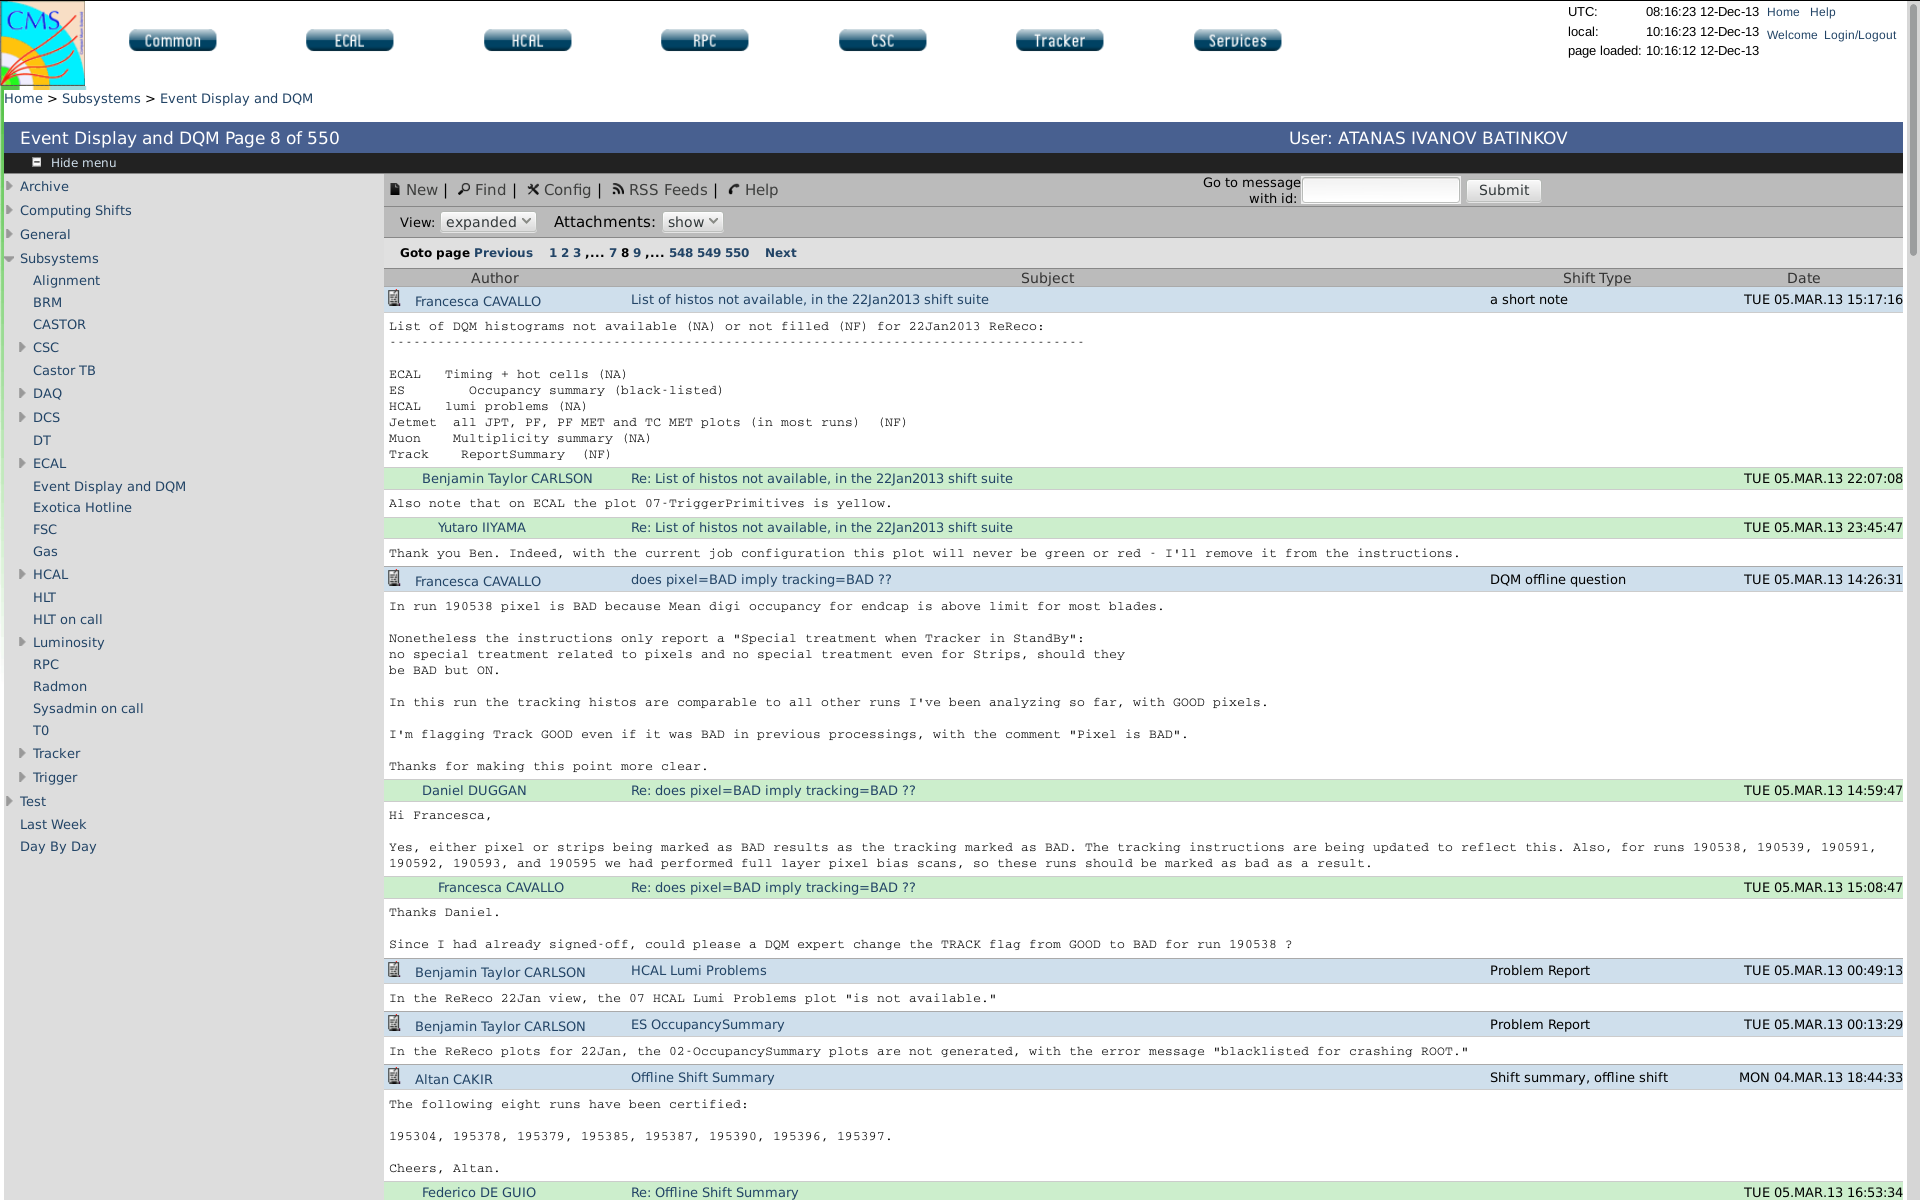
\includegraphics[width=0.5\textwidth, keepaspectratio=true]{Elog.png}
\caption{Elog. In the center a typical Elog usage is shown. All the detector subsystems are organized in sections on the left.}
\label{fig:Elog}
\end{figure}

The DQM on-call coordinates the actions that need to be taken if a problem occurs, and needs to be available 24/7 over the phone and online. The on-call fixes all problems related to the DQM tools and acts as point of contact for all other issues.

\subsection{Improvements in the online}
During the long shutdown 1 of the LHC, many improvements are planned in all the parties of the DQM online realm.

Due to changes introduced to the CMS Data Acquisition System, a full re-implementation of the system that serves data to the DQM online applications is foreseen.

Another enhancement is the addition of publishing capabilities to the online framework. This includes easy access to online databases and CERN/CMS publishing protocols from all the online applications.

Improvements of the monitoring system of the DQM online machines are also planned. Real-time monitoring of the CPU usage, memory consumption, space availability on the hard drives and other aspects will be provided in a central web page.

Compression of the archived online ROOT files is also under investigation. This could reduce the space usage by 50\%. The archive area will be automatically cleaned up to avoid interruptions.

One improvement that will be made to the DQM GUI is the growth of database key from 64 to 128 bit, greatly increasing the index storage. Another is that the database will be split into several pieces - each piece for a different month. This hugely improves the overall robustness of the system because once the month is over the corresponding piece will be reopened in read-only mode and archived, this minimizes the potential loss of data to a single month. Server-client communication improvements are also planned. An increase of the communication speed, compression of the transferred data and even client-side render of the histograms will be introduced. The database also could be migrated to Kyoto cabinet \cite{kyotocabinet} or leveldb \cite{leveldb} if they provide better performance.

The alarm system also will be improved. An easy suppression of the individual errors without interaction from a DQM expert will be added, allowing the shift crew to suppress/enable individual alarms. The error messages may also be extended to provide additional information useful in resolving specific problems.

% needed in second column of first page if using \IEEEpubid
%\IEEEpubidadjcol

\section{DQM offline realm}
The DQM offline system is used for certification of the recorded data. It provides a detailed view of the complete event reconstruction from all recorded data. Only certified data may be used in CMS analyses for publication (Fig. \ref{fig:OfflineChain}).

\begin{figure}
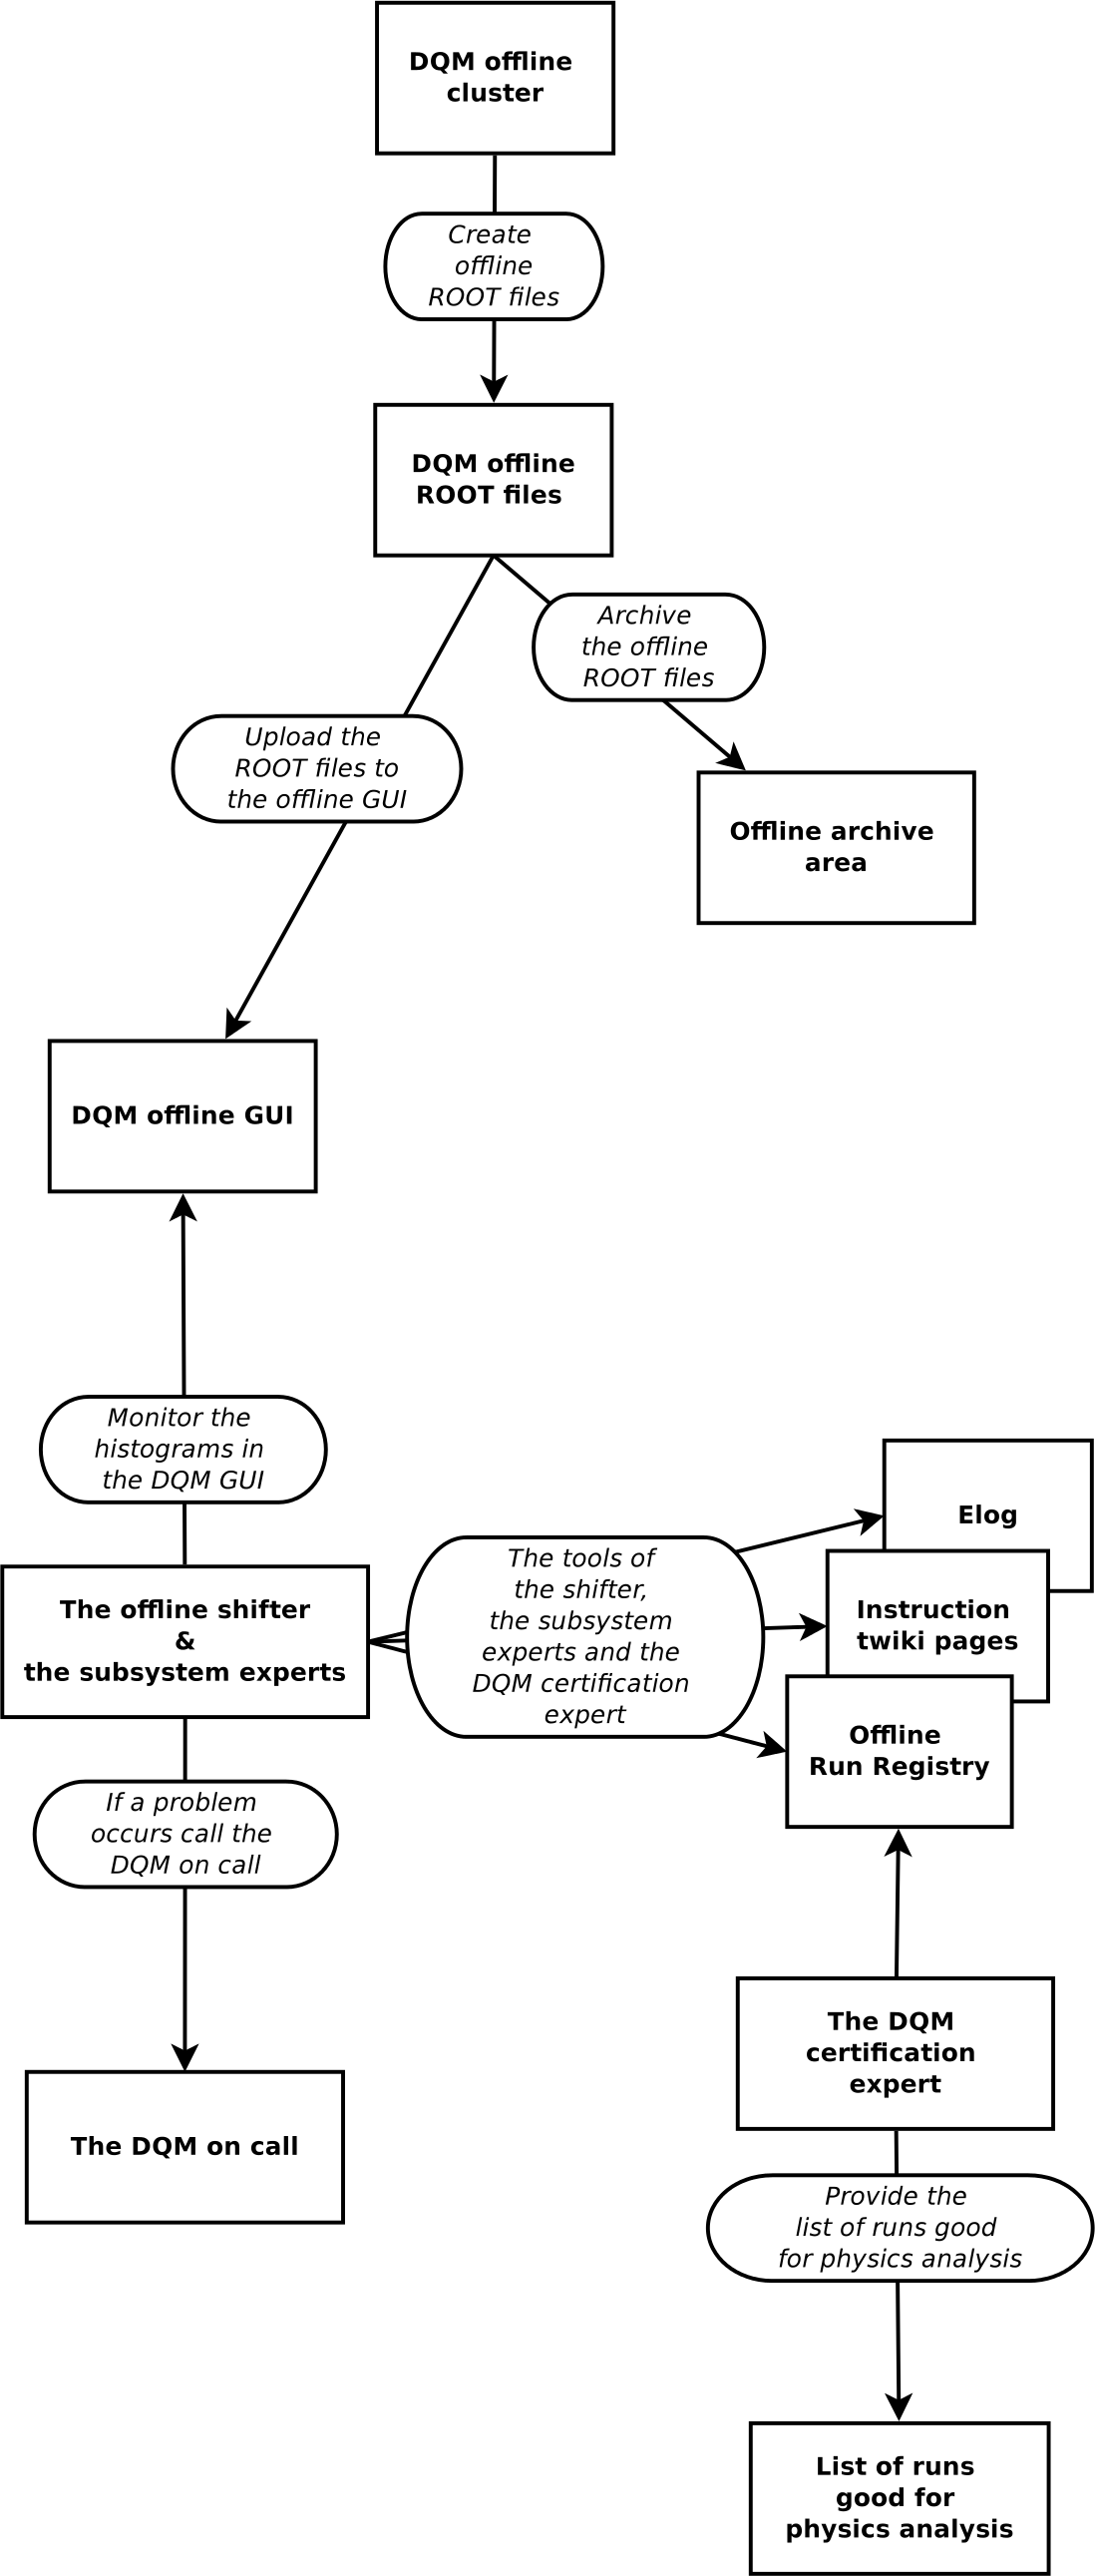
\includegraphics[width=0.5\textwidth, keepaspectratio=true]{OfflineChain.png}
\caption{The DQM offline chain. The figure outlines the main aspects of the offline realm: DQM offline data processing, the offline DQM GUI and offline data certification.}
\label{fig:OfflineChain}
\end{figure}

\subsection{DQM Offline data processing}
The DQM offline data processing runs at CERN’s computing center and produces histograms that are further examined for data to be certified. In the offline all data is processed. This process includes prompt reconstruction as well as detector data analysis. The offline DQM process is split into two steps: the DQM step and the harvesting step. In the DQM step the histograms are created and filled with information from the CMS event data. In the harvesting step the histograms are extracted from the event data files and summed together across the entire run to yield full event statistics. The final results are output to ROOT files, injected into the offline GUI and archived.

\subsection{The offline DQM GUI}
The DQM GUI collects, stores, and visualizes the results from the offline DQM data processing. The GUI shares the same code as the online GUI (for a full list of features and improvements see \ref{sec:OnlineGUI}) but with a different look in the user interface. Online and offline GUIs have their own set of workspaces, layouts and render plug-ins that define their unique look. The offline GUI needs to be even more stable than the online so the deployment schema is more rigid. The installation of new software follows the official releases of an internal CMS group responsible for the web services of the collaboration.

\subsection{The offline data certification}
The offline data certification is performed by three groups: the offline shifter, the subsystem experts and the DQM certification expert. The scope of the DQM offline shift is to produce certifications for various reconstruction iterations. It operate at CERN, FNAL \cite{FNAL} and DESY \cite{DESY}. There are 4 shifts per day and each takes 6 hours. Offline DQM shifts can be scheduled outside of global data taking periods. The offline shifter monitors a subset of histograms for every detector and reconstruction objects in the offline DQM GUI. The tools of the DQM offline shifter are explained in section \ref{sec:OnlineShifter} with the exception that they are tuned for the offline DQM. After the shifter job is done the experts from all subsystems produce certifications for specific detectors or reconstruction algorithms. Finally the DQM certification experts combine the results from the offline shifters and the subsystem experts to provide the list of runs certified as usable for physics analysis.

\subsection{Improvements in the offline}
The framework of the CMS reconstruction software is currently migrating to multi-core, multi-thread data processing. The DQM framework is being adapted to the new processing model. This requires many changes to all the participants in the offline data processing.

% An example of a floating figure using the graphicx package.
% Note that \label must occur AFTER (or within) \caption.
% For figures, \caption should occur after the \includegraphics.
% Note that IEEEtran v1.7 and later has special internal code that
% is designed to preserve the operation of \label within \caption
% even when the captionsoff option is in effect. However, because
% of issues like this, it may be the safest practice to put all your
% \label just after \caption rather than within \caption{}.
%
% Reminder: the "draftcls" or "draftclsnofoot", not "draft", class
% option should be used if it is desired that the figures are to be
% displayed while in draft mode.
%
%\begin{figure}[!t]
%\centering
%\includegraphics[width=2.5in]{myfigure}
% where an .eps filename suffix will be assumed under latex, 
% and a .pdf suffix will be assumed for pdflatex; or what has been declared
% via \DeclareGraphicsExtensions.
%\caption{Simulation Results}
%\label{fig_sim}
%\end{figure}

% Note that IEEE typically puts floats only at the top, even when this
% results in a large percentage of a column being occupied by floats.


% An example of a double column floating figure using two subfigures.
% (The subfig.sty package must be loaded for this to work.)
% The subfigure \label commands are set within each subfloat command, the
% \label for the overall figure must come after \caption.
% \hfil must be used as a separator to get equal spacing.
% The subfigure.sty package works much the same way, except \subfigure is
% used instead of \subfloat.
%
%\begin{figure*}[!t]
%\centerline{\subfloat[Case I]\includegraphics[width=2.5in]{subfigcase1}%
%\label{fig_first_case}}
%\hfil
%\subfloat[Case II]{\includegraphics[width=2.5in]{subfigcase2}%
%\label{fig_second_case}}}
%\caption{Simulation results}
%\label{fig_sim}
%\end{figure*}
%
% Note that often IEEE papers with subfigures do not employ subfigure
% captions (using the optional argument to \subfloat), but instead will
% reference/describe all of them (a), (b), etc., within the main caption.


% An example of a floating table. Note that, for IEEE style tables, the 
% \caption command should come BEFORE the table. Table text will default to
% \footnotesize as IEEE normally uses this smaller font for tables.
% The \label must come after \caption as always.
%
%\begin{table}[!t]
%% increase table row spacing, adjust to taste
%\renewcommand{\arraystretch}{1.3}
% if using array.sty, it might be a good idea to tweak the value of
% \extrarowheight as needed to properly center the text within the cells
%\caption{An Example of a Table}
%\label{table_example}
%\centering
%% Some packages, such as MDW tools, offer better commands for making tables
%% than the plain LaTeX2e tabular which is used here.
%\begin{tabular}{|c||c|}
%\hline
%One & Two\\
%\hline
%Three & Four\\
%\hline
%\end{tabular}
%\end{table}


% Note that IEEE does not put floats in the very first column - or typically
% anywhere on the first page for that matter. Also, in-text middle ("here")
% positioning is not used. Most IEEE journals use top floats exclusively.
% Note that, LaTeX2e, unlike IEEE journals, places footnotes above bottom
% floats. This can be corrected via the \fnbelowfloat command of the
% stfloats package.



\section{Conclusion}
The DQM provides a full end-to-end data quality monitoring system for the CMS experiment. The overall stability has increased with the time and currently the whole system is very robust. Both online and offline chains have been in production for more than 5 years. The code is constantly updated with improvements and new features following the latest software trends. Strong bonds are established between the central DQM framework and the detector subsystems’ applications in order to provide maximum data processing efficiency. The DQM web technology has been a key and very successful part of the CMS experiment, allowing (among many other things) remote access to online and offline data monitoring for experts worldwide. This system has provided the foundation for the highest level of data quality, and with the improvements under way, this effort will provide even higher level of monitoring for CMS as it enters the LHC Run 2 era.


% if have a single appendix:
%\appendix[Proof of the Zonklar Equations]
% or
%\appendix  % for no appendix heading
% do not use \section anymore after \appendix, only \section*
% is possibly needed

% use appendices with more than one appendix
% then use \section to start each appendix
% you must declare a \section before using any
% \subsection or using \label (\appendices by itself
% starts a section numbered zero.)
%


\appendices
% \section{Proof of the First Zonklar Equation}
% Appendix one text goes here.

% you can choose not to have a title for an appendix
% if you want by leaving the argument blank
% \section{}
% Appendix two text goes here.


% use section* for acknowledgement
\section*{Acknowledgment}
\hyphenation{Bundes-ministerium Forschungs-gemeinschaft Forschungs-zentren} We congratulate our colleagues in the CERN accelerator departments for the excellent performance of the LHC and thank the technical and administrative staffs at CERN and at other CMS institutes for their contributions to the success of the CMS effort. In addition, we gratefully acknowledge the computing centres and personnel of the Worldwide LHC Computing Grid for delivering so effectively the computing infrastructure essential to our analyses. Finally, we acknowledge the enduring support for the construction and operation of the LHC and the CMS detector provided by the following funding agencies: the Austrian Federal Ministry of Science and Research and the Austrian Science Fund; the Belgian Fonds de la Recherche Scientifique, and Fonds voor Wetenschappelijk Onderzoek; the Brazilian Funding Agencies (CNPq, CAPES, FAPERJ, and FAPESP); the Bulgarian Ministry of Education and Science; CERN; the Chinese Academy of Sciences, Ministry of Science and Technology, and National Natural Science Foundation of China; the Colombian Funding Agency (COLCIENCIAS); the Croatian Ministry of Science, Education and Sport; the Research Promotion Foundation, Cyprus; the Ministry of Education and Research, Recurrent financing contract SF0690030s09 and European Regional Development Fund, Estonia; the Academy of Finland, Finnish Ministry of Education and Culture, and Helsinki Institute of Physics; the Institut National de Physique Nucl\'eaire et de Physique des Particules~/~CNRS, and Commissariat \`a l'\'Energie Atomique et aux \'Energies Alternatives~/~CEA, France; the Bundesministerium f\"ur Bildung und Forschung, Deutsche Forschungsgemeinschaft, and Helmholtz-Gemeinschaft Deutscher Forschungszentren, Germany; the General Secretariat for Research and Technology, Greece; the National Scientific Research Foundation, and National Innovation Office, Hungary; the Department of Atomic Energy and the Department of Science and Technology, India; the Institute for Studies in Theoretical Physics and Mathematics, Iran; the Science Foundation, Ireland; the Istituto Nazionale di Fisica Nucleare, Italy; the Korean Ministry of Education, Science and Technology and the World Class University program of NRF, Republic of Korea; the Lithuanian Academy of Sciences; the Mexican Funding Agencies (CINVESTAV, CONACYT, SEP, and UASLP-FAI); the Ministry of Business, Innovation and Employment, New Zealand; the Pakistan Atomic Energy Commission; the Ministry of Science and Higher Education and the National Science Centre, Poland; the Funda\c{c}\~ao para a Ci\^encia e a Tecnologia, Portugal; JINR, Dubna; the Ministry of Education and Science of the Russian Federation, the Federal Agency of Atomic Energy of the Russian Federation, Russian Academy of Sciences, and the Russian Foundation for Basic Research; the Ministry of Education, Science and Technological Development of Serbia; the Secretar\'{\i}a de Estado de Investigaci\'on, Desarrollo e Innovaci\'on and Programa Consolider-Ingenio 2010, Spain; the Swiss Funding Agencies (ETH Board, ETH Zurich, PSI, SNF, UniZH, Canton Zurich, and SER); the National Science Council, Taipei; the Thailand Center of Excellence in Physics, the Institute for the Promotion of Teaching Science and Technology of Thailand, Special Task Force for Activating Research and the National Science and Technology Development Agency of Thailand; the Scientific and Technical Research Council of Turkey, and Turkish Atomic Energy Authority; the Science and Technology Facilities Council, UK; the US Department of Energy, and the US National Science Foundation.

Individuals have received support from the Marie-Curie programme and the European Research Council and EPLANET (European Union); the Leventis Foundation; the A. P. Sloan Foundation; the Alexander von Humboldt Foundation; the Belgian Federal Science Policy Office; the Fonds pour la Formation \`a la Recherche dans l'Industrie et dans l'Agriculture (FRIA-Belgium); the Agentschap voor Innovatie door Wetenschap en Technologie (IWT-Belgium); the Ministry of Education, Youth and Sports (MEYS) of Czech Republic; the Council of Science and Industrial Research, India; the Compagnia di San Paolo (Torino); the HOMING PLUS programme of Foundation for Polish Science, cofinanced by EU, Regional Development Fund; and the Thalis and Aristeia programmes cofinanced by EU-ESF and the Greek NSRF.


% Can use something like this to put references on a page
% by themselves when using endfloat and the captionsoff option.
\ifCLASSOPTIONcaptionsoff
  \newpage
\fi



% trigger a \newpage just before the given reference
% number - used to balance the columns on the last page
% adjust value as needed - may need to be readjusted if
% the document is modified later
%\IEEEtriggeratref{8}
% The "triggered" command can be changed if desired:
%\IEEEtriggercmd{\enlargethispage{-5in}}

% references section

% can use a bibliography generated by BibTeX as a .bbl file
% BibTeX documentation can be easily obtained at:
% http://www.ctan.org/tex-archive/biblio/bibtex/contrib/doc/
% The IEEEtran BibTeX style support page is at:
% http://www.michaelshell.org/tex/ieeetran/bibtex/
%\bibliographystyle{IEEEtran}
% argument is your BibTeX string definitions and bibliography database(s)
%\bibliography{IEEEabrv,../bib/paper}
%
% <OR> manually copy in the resultant .bbl file
% set second argument of \begin to the number of references
% (used to reserve space for the reference number labels box)
\begin{thebibliography}{1}
\bibitem{CHEP13}
The CMS Data Quality Monitoring software: experience and future improvements, F. De Guio et al, CHEP13

\bibitem{CHEP09}
CMS data quality monitoring: systems and experiences, L. Tuura et al, CHEP09

\bibitem{LHC}
LHC Machine, JINST 3 S08001, 2008

\bibitem{CERN}
http://home.web.cern.ch/

\bibitem{CMS}
The CMS Experiment at the CERN LHC, JINST 3 S08004, 2008.

\bibitem{ROOT}
http://root.cern.ch/drupal/

\bibitem{kyotocabinet}
http://fallabs.com/kyotocabinet/

\bibitem{leveldb}
https://code.google.com/p/leveldb/

\bibitem{FNAL}
https://www.fnal.gov/

\bibitem{DESY}
http://www.desy.de/

\end{thebibliography}

% biography section
% 
% If you have an EPS/PDF photo (graphicx package needed) extra braces are
% needed around the contents of the optional argument to biography to prevent
% the LaTeX parser from getting confused when it sees the complicated
% \includegraphics command within an optional argument. (You could create
% your own custom macro containing the \includegraphics command to make things
% simpler here.)
%\begin{biography}[{\includegraphics[width=1in,height=1.25in,clip,keepaspectratio]{mshell}}]{Michael Shell}
% or if you just want to reserve a space for a photo:

% \begin{IEEEbiography}{Michael Shell}
% Biography text here.
% \end{IEEEbiography}

% if you will not have a photo at all:
% \begin{IEEEbiographynophoto}{John Doe}
% Biography text here.
% \end{IEEEbiographynophoto}

% insert where needed to balance the two columns on the last page with
% biographies
%\newpage

% \begin{IEEEbiographynophoto}{Jane Doe}
% Biography text here.
% \end{IEEEbiographynophoto}

% You can push biographies down or up by placing
% a \vfill before or after them. The appropriate
% use of \vfill depends on what kind of text is
% on the last page and whether or not the columns
% are being equalized.

%\vfill

% Can be used to pull up biographies so that the bottom of the last one
% is flush with the other column.
%\enlargethispage{-5in}



% that's all folks
\end{document}
